\chapter{Implementation}
\label{cha:implementation}
In the implementation phase, the solution developed in the various domains is
implemented into the target platforms, accordingly to the system design
specification. In this chapter is presented the implementation for the various
domains and subsystems identified, namely the \texttt{Remote Client},
\texttt{Remote Server} and
\texttt{Local System}.

\section{Hardware}
\label{sec:hw-imp}

The implementation of the hardware consists on mount everything that was bought and created and finish with the final prototype.
This final prototype consists in a box with all the hardware inside of it, as it can be seen on fig~\ref{fig:hw-imp}.
This also means that inside that box is the designed \gls{pcb} (fig~\ref{fig:pcb}).
\begin{figure}
\centering
  %
  \begin{subfigure}{.4\textwidth}
  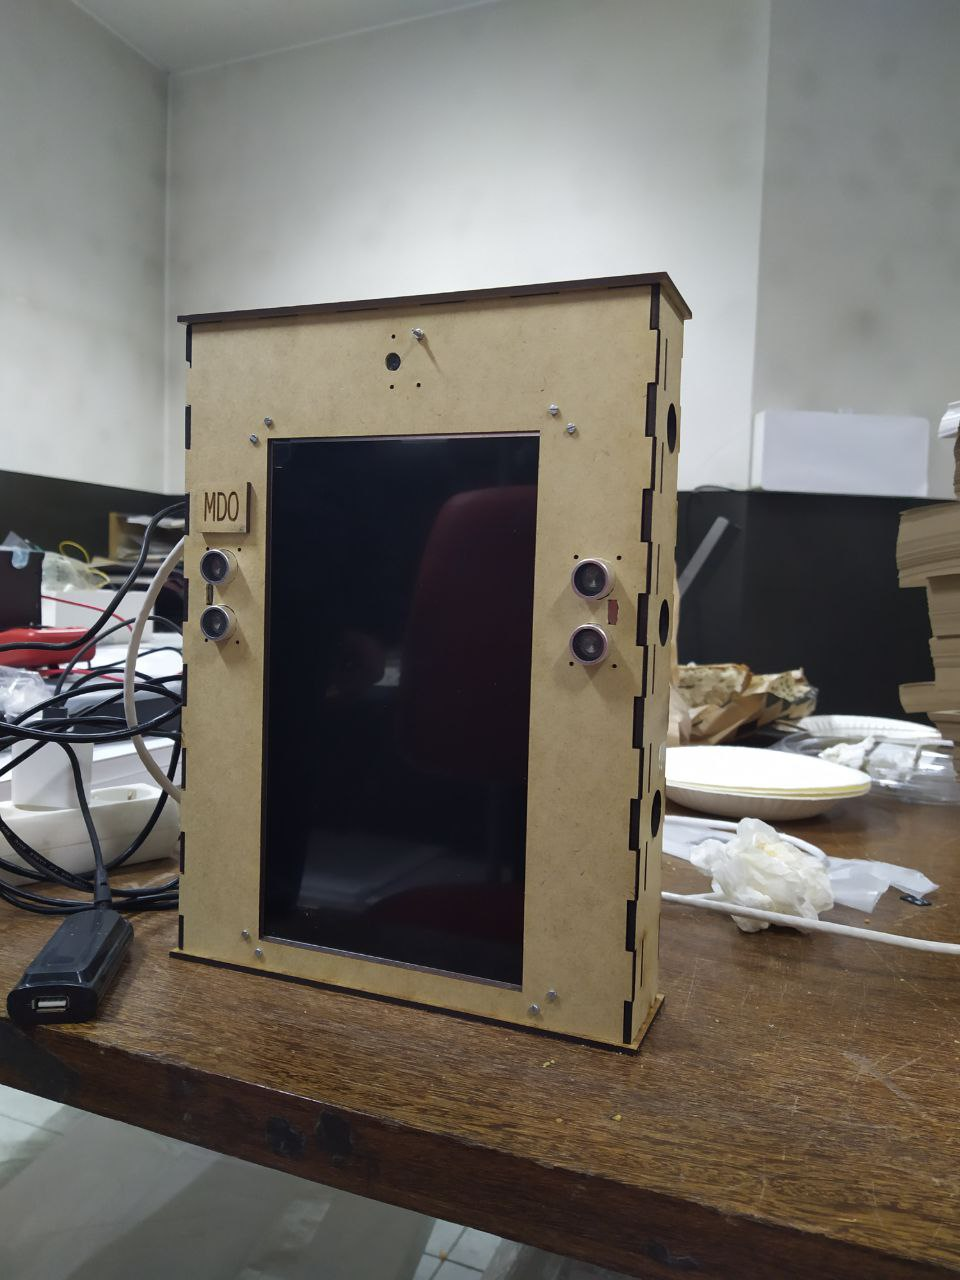
\includegraphics[width=\textwidth]{img/hw-all.jpg}%
  \caption{Login View}%
  \label{fig:hw-all}
\end{subfigure}
%
  \begin{subfigure}{.4\textwidth}
    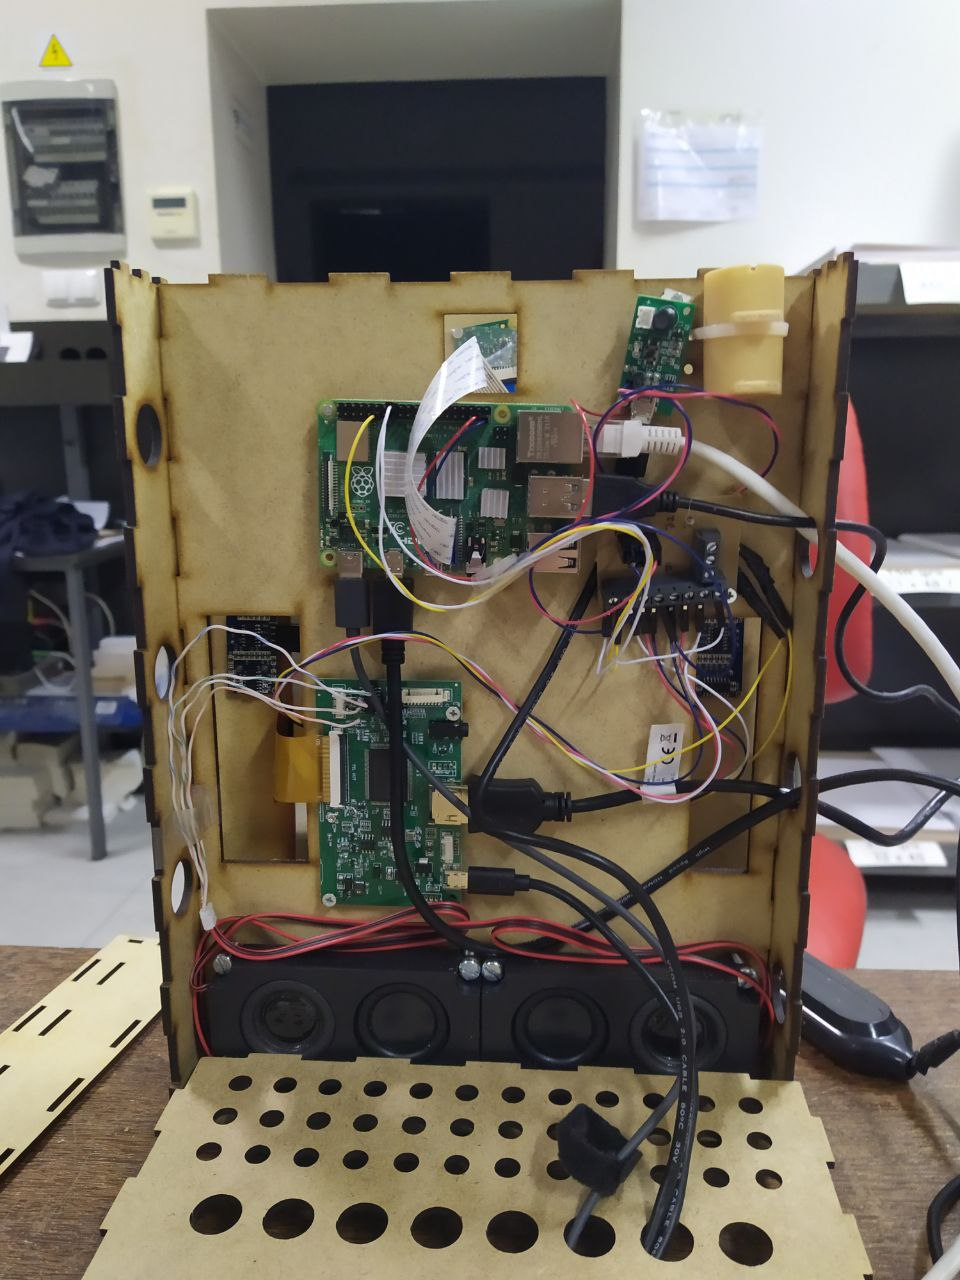
\includegraphics[width=\textwidth]{img/hw-inside.jpg}%
  \caption{Final Hardware Implementation}%
  \label{fig:hw-inside}
  \end{subfigure}
  % 
  \caption{MainWindow views}%
  \label{fig:hw-imp}
\end{figure}
%
\begin{figure}[!htb]
    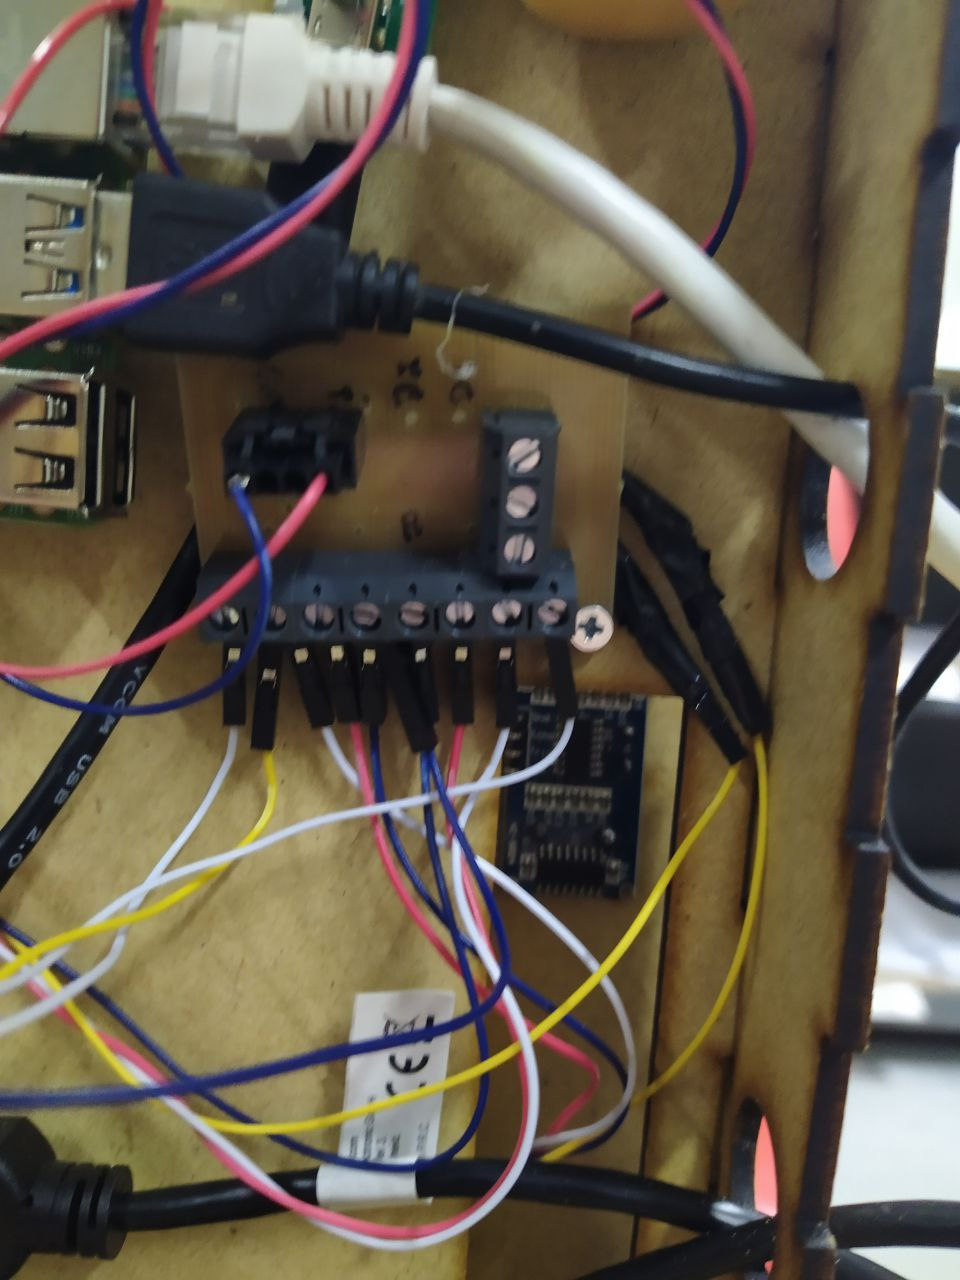
\includegraphics[width=.5\textwidth]{img/pcb.jpg}%
  \caption{Final \gls{pcb}}%
  \label{fig:pcb}
  \end{figure}
%%% Local Variables:
%%% mode: latex
%%% TeX-master: "../../../dissertation"
%%% End:

\section{Remote Client}
\label{sec:rc}
%
The \gls{mdo-rc} is a Desktop application that is developed in QT.
This application handles all the job that is referred to interaction between this last and a \textbf{brand} - to rent an ad or see its statistics - or an \textbf{admin} - to manage all users, stations and ads.

\subsection{Classes}
\label{sub-sec:classes}
%
For a more easier developing, the layout and implementation of this application was divided by 3 distinct \texttt{QWidget} classes:
\begin{enum-c}
\item \texttt{MainWindow} class -- to handle the login and register use cases;
\item \texttt{BrandWindow} class -- to handle everything related to the brand usage;
\item \texttt{AdminWindow} class -- to handle everything related to the admin usage;
\end{enum-c}

\subsubsection{MainWindow class}
%
The \texttt{MainWindow} class is, as it suggests, the main class of all the program.
This class handles all the transitions between views, such as \emph{Login View}, \emph{Admin View}, \emph{Brand View} and \emph{Register View}.

As it can be seen in the header file of this class (listing \ref{lst:mainwindow-h}), there are two pointers to the other two classes, each one of them as a pointer, in order to be instantiated right on the constructor.
The \texttt{Sess *sess} that refers to the \textbf{MySQL session}, the variables associated with threads and the timer will be explaine later on the next section, as well as some functions like thread functions.
%
\lstinputlisting[language=c++, caption={Declaration of MainWindow class},label=lst:mainwindow-h,
style=customc]{./listing/rc-mainwindow.h}%

All the function with the prefix \texttt{"on\_"} on it are private slots that are created to response to the click of some buttons.

Now, looking at the implementation of the Constructor:

\lstinputlisting[language=c++, firstline=25, lastline = 102, caption={Implementation of the constructor \texttt{MainWindow}},label=lst:mainwindow-imp,
style=customc]{./listing/rc-mainwindow.cpp}%

As it can be seen in Listing \ref{lst:mainwindow-imp}, there's an enumerator that helps the class to navigate through the views.
That's because that management is made with the help of \texttt{Stacked Widgets}.
The \textbf{Main Window} also has a pointer to a stacked widget in order to switch between classes and show different views.

In resume, the main steps to have in considering for the \textbf{Remote Client} part are:
\begin{item-c}
\item Initialization of the session to connect to MySQL server;
\item Instantiation of the other two classes;
\item Signals connections to return back to the Main Window after a logout in each class. 
\end{item-c}

\paragraph{\emph{Layout}}
Fig.~\ref{fig:mw-login-view} and fig.~\ref{fig:mw-register-view} show respectively the Login and Register Views.

These two views interact with help of the database. 
For example, when registering a user, if every parameter is correctly inserted, it will be queued a message to MySQL inserting a new User with \textbf{default brand privilege}.
For the example of logging in, it will be made a queue to the MySQL server asking for a row that matches de inputted username and password and if so, the user will be redirectioned to the specific view according to its privileges.

\begin{figure}[htb!]
  \centering
  %
  \begin{subfigure}{.6\textwidth}
  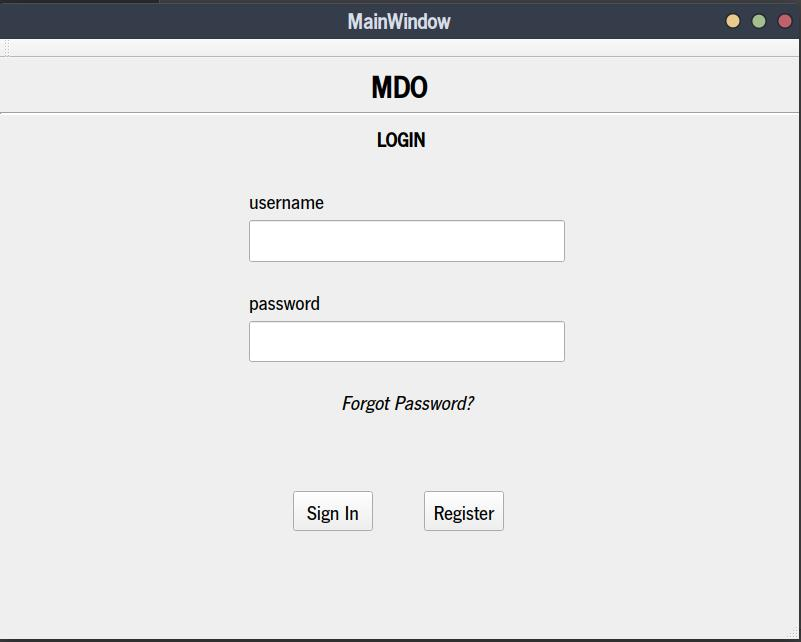
\includegraphics[width=\textwidth]{img/mw-login-view.jpg}%
  \caption{Login View}%
  \label{fig:mw-login-view}
\end{subfigure}

%\hspace{.1\textwidth}
%
  \begin{subfigure}{.6\textwidth}
    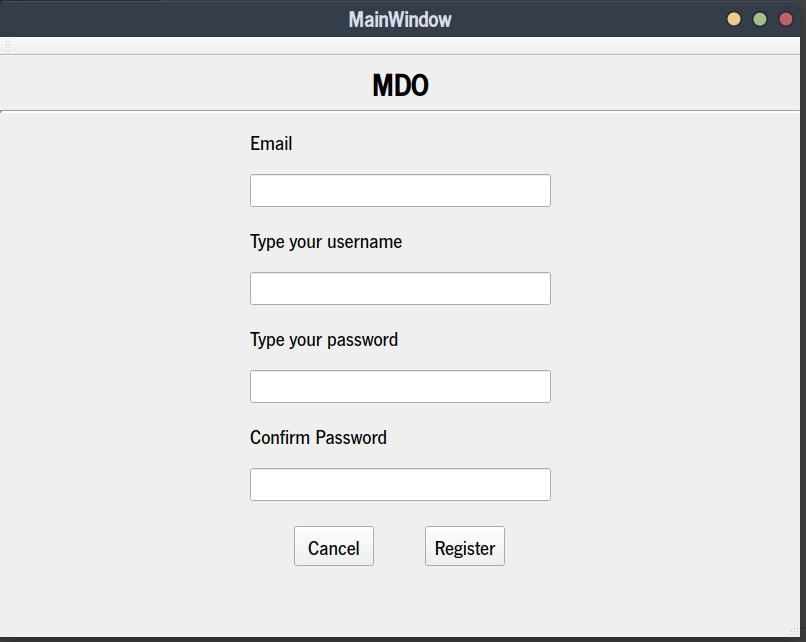
\includegraphics[width=\textwidth]{img/mw-register-view.jpg}%
  \caption{Register View}%
  \label{fig:mw-register-view}
  \end{subfigure}
  % 
  \caption{MainWindow views}%
  \label{fig:ptp-test}
\end{figure}  

\subsubsection{BrandWindow class}
%
The \texttt{BrandWindow} class is, as it suggests, the class that handles all of the brand's features.
This class handles all the transitions between views, such as \emph{Rent Ad View}, \emph{To Rent View} and \emph{Logout} - emits a signal to go back to login.
%
\lstinputlisting[language=c++, caption={Declaration of BrandWindow class},label=lst:brandwindow.h,
style=customc]{./listing/rc-brandwindow.h}%

As it can be seen in the header file of this class (listing \ref{lst:brandwindow.h}), there's also the session to handle the MySQL server connection (\texttt{Sess* sess}), a \texttt{QFileInfo} to handle the files to upload on an Ad and the \texttt{user\_id} which refers to the user that is currently using the app.
As in every part of the code, here there's also the usage of queues to the MySQL server, to rent ads and to see the ads rented to watch its statistics.
In order to make everything more simpler, in the \texttt{Rent View} it is only possible to rent for a range of one week. All the time slots that are already rented appear with a "Rented" \texttt{std::string} and the days that do not correspond to the time space available to rent appear with the label "Unavailable".

Perhaps, one of the most difficult functions to implement was the rent function, that's because it is necessary to add many rows to different tables in order to build a complete Ad on the database, this means that if something went wrong in the middle of the execution, it is necessary to do the inverse process to delete the already inserted rows, because they will not have a link to every tables.

Listing \ref{lst:rent-ad} shows the rent ad function.
%
\lstinputlisting[language=c++, firstline = 341, lastline=462, caption={Implementation of rent function on BrandWindow class},label=lst:rent-ad,
style=customc]{./listing/rc-brandwindow.cpp}

Because of the length and process capability of this function, every little mistake can take to serious consequences, so, it is mandatory to make all and every validation in order to avoid every mistake in the MySQL queue messages. Common errors can be such like redundant blocs of data, or even just a single piece of data.

\paragraph{\emph{Layout}}

Figures \ref{fig:brand-main-view}, \ref{fig:brand-to-rent-view} and \ref{fig:brand-rented-view} show the layout used for all the Brand Views.

\begin{figure}[htb!]
  \centering
  %
  \begin{subfigure}{.4\textwidth}
  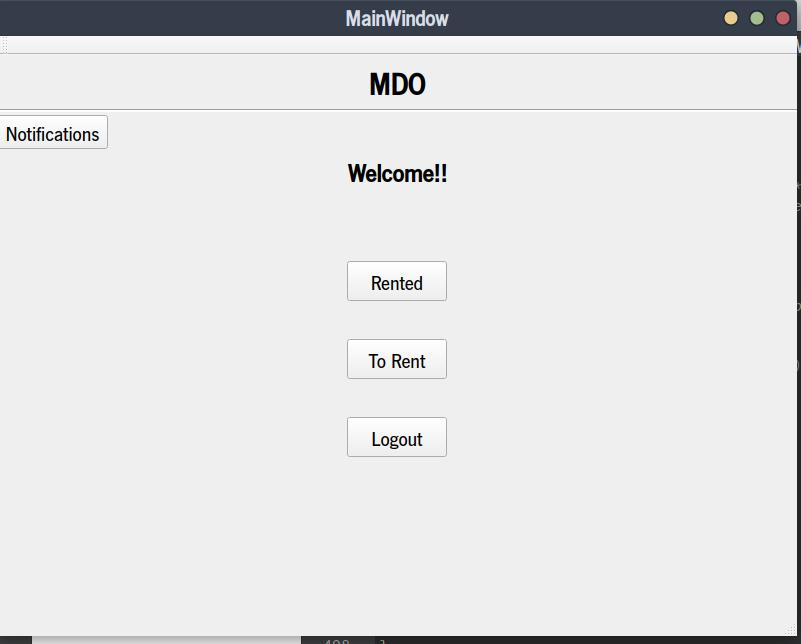
\includegraphics[width=\textwidth]{img/brand-main-view.jpg}%
  \caption{Brand Main View}%
  \label{fig:brand-main-view}
\end{subfigure}

%\hspace{.1\textwidth}
%
  \begin{subfigure}{.4\textwidth}
    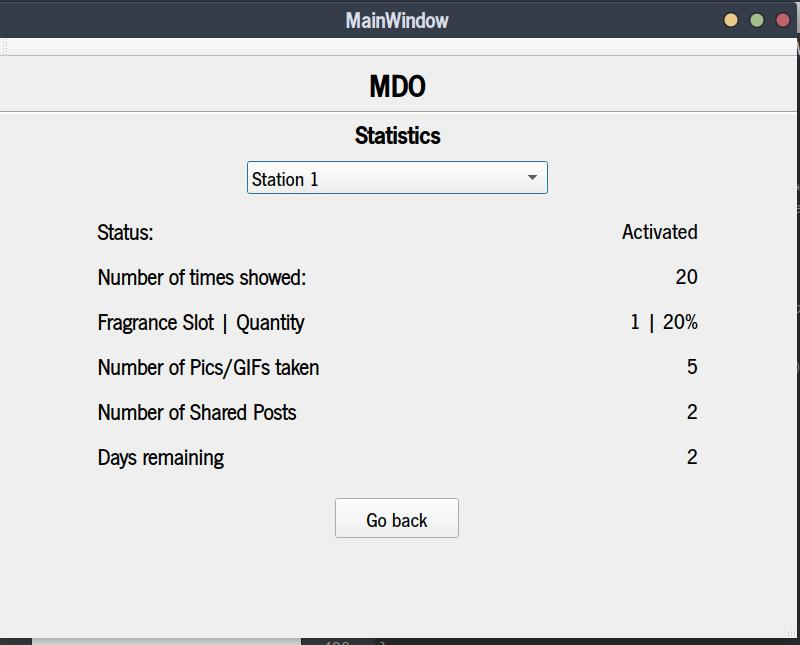
\includegraphics[width=\textwidth]{img/brand-rented-view.jpg}%
  \caption{Brand Rented View}%
  \label{fig:brand-rented-view}
  \end{subfigure}
  % 
  \begin{subfigure}{.4\textwidth}
    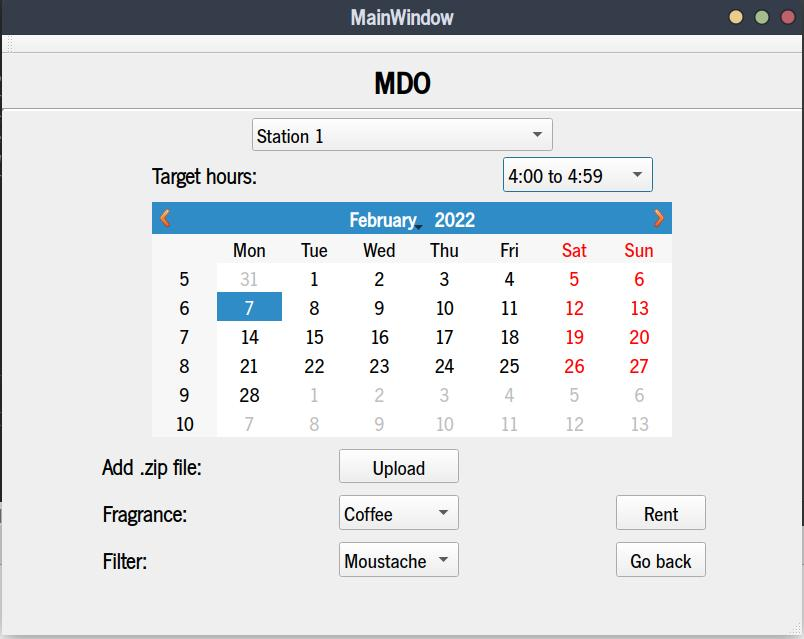
\includegraphics[width=\textwidth]{img/brand-to-rent-view.jpg}%
  \caption{Brand To Rent View}%
  \label{fig:brand-to-rent-view}
  \end{subfigure}
  % 
  \caption{BrandWindow views}%
  \label{fig:ptp-test}
\end{figure} 

\subsubsection{AdminWindow class}
%
The \texttt{AdmindWindow} class is, as it suggests, the class that handles all of the admin's features.
This class handles all the transitions between views, such as \emph{Statistics View}, \emph{Manage Users View}, \emph{Ads To Activate View} and \emph{Test Operation View}.
%
\lstinputlisting[language=c++, caption={Declaration of AdminWindow class},label=lst:adminwindow.h,
style=customc]{./listing/rc-adminwindow.h}%

In terms of private attributes, this class is similar to the \texttt{BrandWindow} class: it has a \texttt{Sess *sess} to handle the communication to MySQL server and it also has a \texttt{user\_id} to know which user is using the app.

Unfortunately, in this case it could not be implemented the Test Operation View because of reasons that will be explained in the next section.

As always, there's a lot of message queues to MySQL in order to handle all the data and shoe them in the \gls{mdo-rc}.
The most interesting feature in this class is the \textbf{Manage Users} function. In this view it is possible to change the permissions of a user, turning into an Admin or a Brand in just a click. It is also possible to delete users, which can be helpful to delete some bots or even users with bad conduct.
Also, the \textbf{Ads to Activate} is an interesting feature, because it can turn ads into active mode or, if denied, it can remove them. This feature is important once it is important to validate all data that is going to be sent to the machines, in order to avoid some type of non-advertisement videos that could appear in the stations.

Listing \ref{lst:admin-manage-users} shows the function \textbf{Manage Users}.
%
\lstinputlisting[language=c++, firstline=273, lastline=306, caption={Implementation of Manage Users from AdminWindow class},label=lst:admin-manage-users,
style=customc]{./listing/rc-adminwindow.cpp}%

Listing \ref{lst:admin-ads-to-act} shows the \textbf{Ads to Activate} feature.
%
\lstinputlisting[language=c++, firstline=376, lastline=430, caption={Implementation of Ads TO Activate from AdminWindow class},label=lst:admin-ads-to-act,
style=customc]{./listing/rc-adminwindow.cpp}%

\paragraph{\emph{Layout}}
%
On figures \ref{fig:admin-main-view}, \ref{fig:admin-manage-users-view} and \ref{fig:admin-ads-to-act-view} are all the views from the Admin Views.

\begin{figure}[htb!]
  \centering
  %
  \begin{subfigure}{.4\textwidth}
  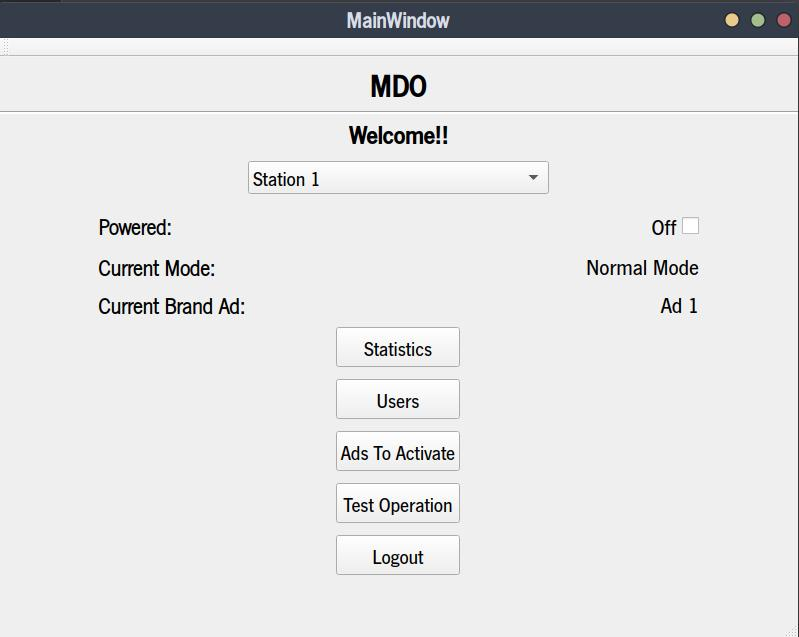
\includegraphics[width=\textwidth]{img/admin-main-view.jpg}%
  \caption{Admin Main View}%
  \label{fig:admin-main-view}
\end{subfigure}

%\hspace{.1\textwidth}
%
  \begin{subfigure}{.4\textwidth}
    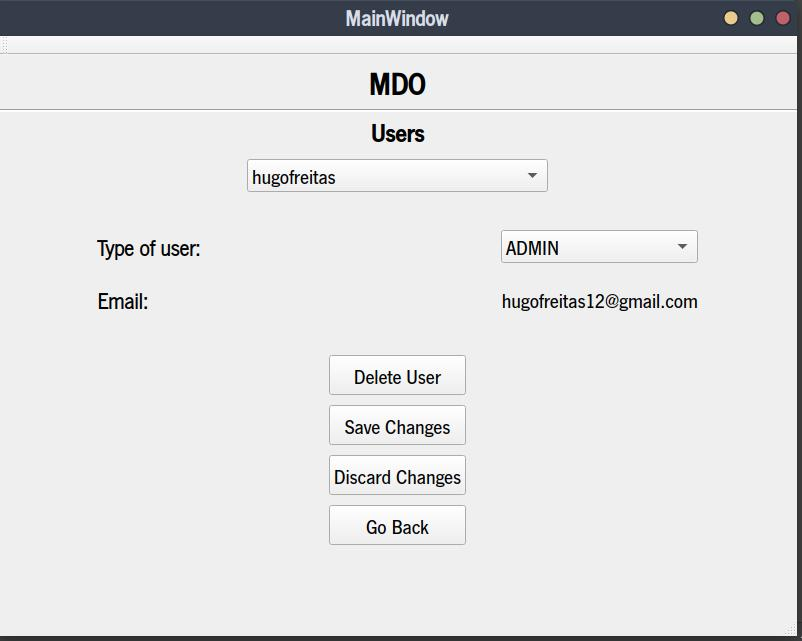
\includegraphics[width=\textwidth]{img/admin-manage-users-view.jpg}%
  \caption{Manage Users View}%
  \label{fig:admin-manage-users-view}
  \end{subfigure}
  % 
  \begin{subfigure}{.4\textwidth}
    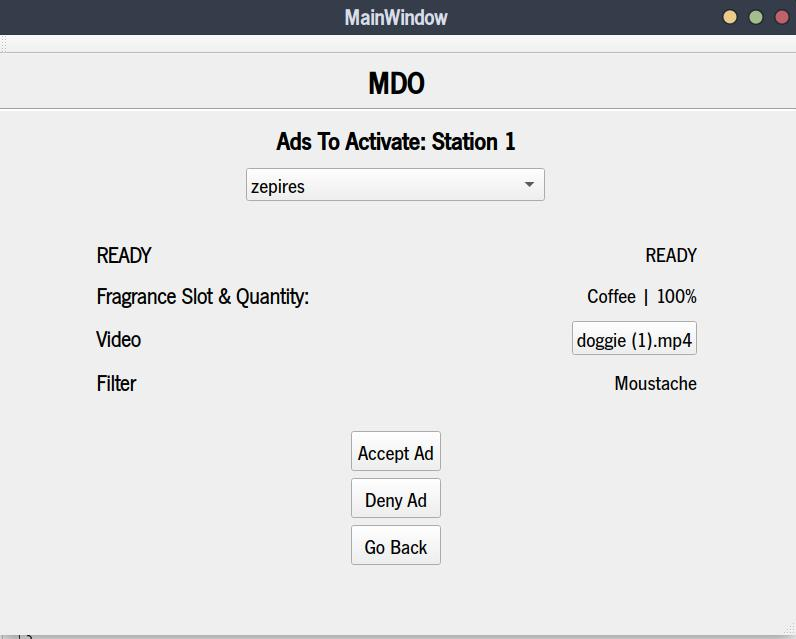
\includegraphics[width=\textwidth]{img/admin-ads-to-act.jpg}%
  \caption{Ads To Activate View}%
  \label{fig:admin-ads-to-act-view}
  \end{subfigure}
  % 
  \caption{AdminWindow views}%
  \label{fig:ptp-test}
\end{figure} 
\section{Remote Server}
\label{sec:rs}
%
The \gls{mdo-rs} was one of the subsystems previously designed to be implemented.
This application would give a more distributed architecture to the overall system.

Unfortunately, because of laps in time spent trying to resolve some unexpected issues and for many other variants, it turned out that it was not possible to develop a real Remote Server.
So, in terms to make everything work at its minimums, it was implemented a "kind of" Remote Server in the Remote Client.
This improvised Remote Server has a full database running in MySQL Server (as it could be seen before) and it has threads to create connections with clients - in this case, local systems - and send to them the information needed, such as new Ads information.

\subsection{Data Base}
The Data Base is one of the most important parts of this system for obvious reasons: this keeps all data stored and easy to access from the Remote Client and the Remote server.
Throughout its implementation, it suffered various iterations that were being stored in two different scripts, these scripts are \texttt{init.txt} (that initializes the Data Base) and \texttt{insert-values.txt} that populates the Data Base.
Implementing it by this way made everything more easy to develop because if it were errors on the Data Base, it was very fast to drop it, create it and populate it again.

Listing \ref{lst:init-sql} shows the init script to create the database.
%
\lstinputlisting[language=c++, caption={Script to create Data Base},label=lst:init-sql,
style=customc]{./listing/init.txt}%

Listing \ref{lst:populate-sql} shows the init script to create the database.
%
\lstinputlisting[language=c++, caption={Script to populate Data Base},label=lst:populate-sql,
style=customc]{./listing/init.txt}%

 

\subsection{Threads}
Looking back to Listing \ref{lst:mainwindow-h}, the threads that are being used are:
\begin{item-c}
\item \texttt{server\_thr} -- used to receive connections from other systems;
\item \texttt{receive\_from\_ls\_thr} -- used to receive messages from other systems;
\item \texttt{send\_to\_ls\_thr} -- used to send data to local system;
\item \texttt{update\_local\_system\_thr} -- updates the local system periodically.
\end{item-c}

\subsubsection{server\_thr}
In listing \ref{lst:server-thr} it is possible to take a look to the thread that waits for the connection of the local system.
%
\lstinputlisting[language=c++, firstline=413, lastline=463, caption={Implementation of Server Thread},label=lst:server-thr,
style=customc]{./listing/rc-mainwindow.cpp}%

This function creates a socket with a default port and starts the binding.
After a successes on binding, the thread blocks on \texttt{listen} to listen for an incoming connection.
As soon as it comes an incoming connection, the thread accepts it and runs the functions \texttt{connectionEneable} and stores the socket in order to keep the communication and signalize other functions that they can start sharing content with the local system.

\subsubsection{receive\_from\_ls\_thr}
In listing \ref{lst:recv-from-ls} is the implementation of the thread that receives messages from the local system.
%
\lstinputlisting[language=c++, firstline=492, lastline=505, caption={Implementation of Receive from \gls{mdo-l} Thread},label=lst:recv-from-ls,
style=customc]{./listing/rc-mainwindow.cpp}%

The function wait for the server to be connected to the local system, once that connection is established it blocks on the \texttt{recv}, waiting to receive something from the previously stored socket.

\subsubsection{send\_to\_ls\_thr}
Listing \ref{lst:send-to-ls} shows how the thread to send data to the local system works
%
\lstinputlisting[language=c++, firstline=507, lastline=530, caption={Implementation of Send to \gls{mdo-l} Thread},label=lst:send-to-ls,
style=customc]{./listing/rc-mainwindow.cpp}%

Firstly, as in the previous thread, it waits until connection is established. After that, it waits for a conditional signal that is sent when a timer expires. When that signal triggers to HIGH, it creates a frame to send that will be interpreted by the local system.

\subsubsection{update\_local\_system\_thr}
This function waits for a conditional signal to continue executing. This conditional signal is set when a timer expires, after that it jumps to the function \texttt{upload\_and\_update} that uploads the file with \texttt{curlpp} and then signalizes the previous function to execute.
%
\lstinputlisting[language=c++, firstline=264, lastline=288, caption={Implementation of Update \gls{mdo-l} Thread},label=lst:updt-ls,
style=customc]{./listing/rc-mainwindow.cpp}%

Obviously, this was the fastest way used to implement a Remote Server, encapsulating it in the Remote Client. In the future, all these threads will leave this app and will migrate and be adjusted to work in a more expandable and robust way.
\section{Local System}
\label{sec:local-system-1}
In this section, the local system implementation is discussed, walking through
its most fundamental aspects.

\subsection{Buildroot configuration}
\label{sec:buildr-conf}
Buildroot is a tool to build custom tailored embedded Linux systems through
cross-compilation, easing the creation and deployment of such systems to be
loaded in the target system.
The base configuration resides in the Buildroot installation path. As a first
step the default configuration for a specific target must be generated running
\texttt{make <TARGET\_ARCH\_defconfig>}. Then, \texttt{make menuconfig} can be
executed to provide a \gls{gui} to interface the configurations of the custom
embedded Linux image.

The fundamental configurations for the project are:
\begin{item-c}
\item \emph{system configuration}: Enabling root login with password; Run a login
  prompt after boot;
\item \emph{filesystem images}: selection of file format and size for the image;
\item \emph{Toolchain}: setup of the development toolchain for the target,
  defining the C library and thread library debugging.
\item \emph{Network}: setup of the network utilities such as \texttt{dropbear}
  and \texttt{dhcpd} to ease the \gls{tcp-ip} communication with the target.
\item \emph{Packages}: setup of the relevant packages for the project, namely,
  \texttt{opencv4} for image acquisition and processing, \texttt{Qt} for
  \gls{ui}, \texttt{libcurl} to download ads, and \texttt{libcamera} to
  interface the \gls{csi} camera of the Raspberry Pi. 
\end{item-c}

After setting the \texttt{Buildroot} configurations, the target image is
generated using \texttt{make} and, if successful, it can be loaded into the
target platform.


Fig.~\ref{fig:build-cfg-4} through Fig.~\ref{fig:buildroot-cfg-4} presents the
Buildroot setup of some features using the \texttt{make menuconfig} utility.
% 
\begin{figure}[htb!]
\centering
    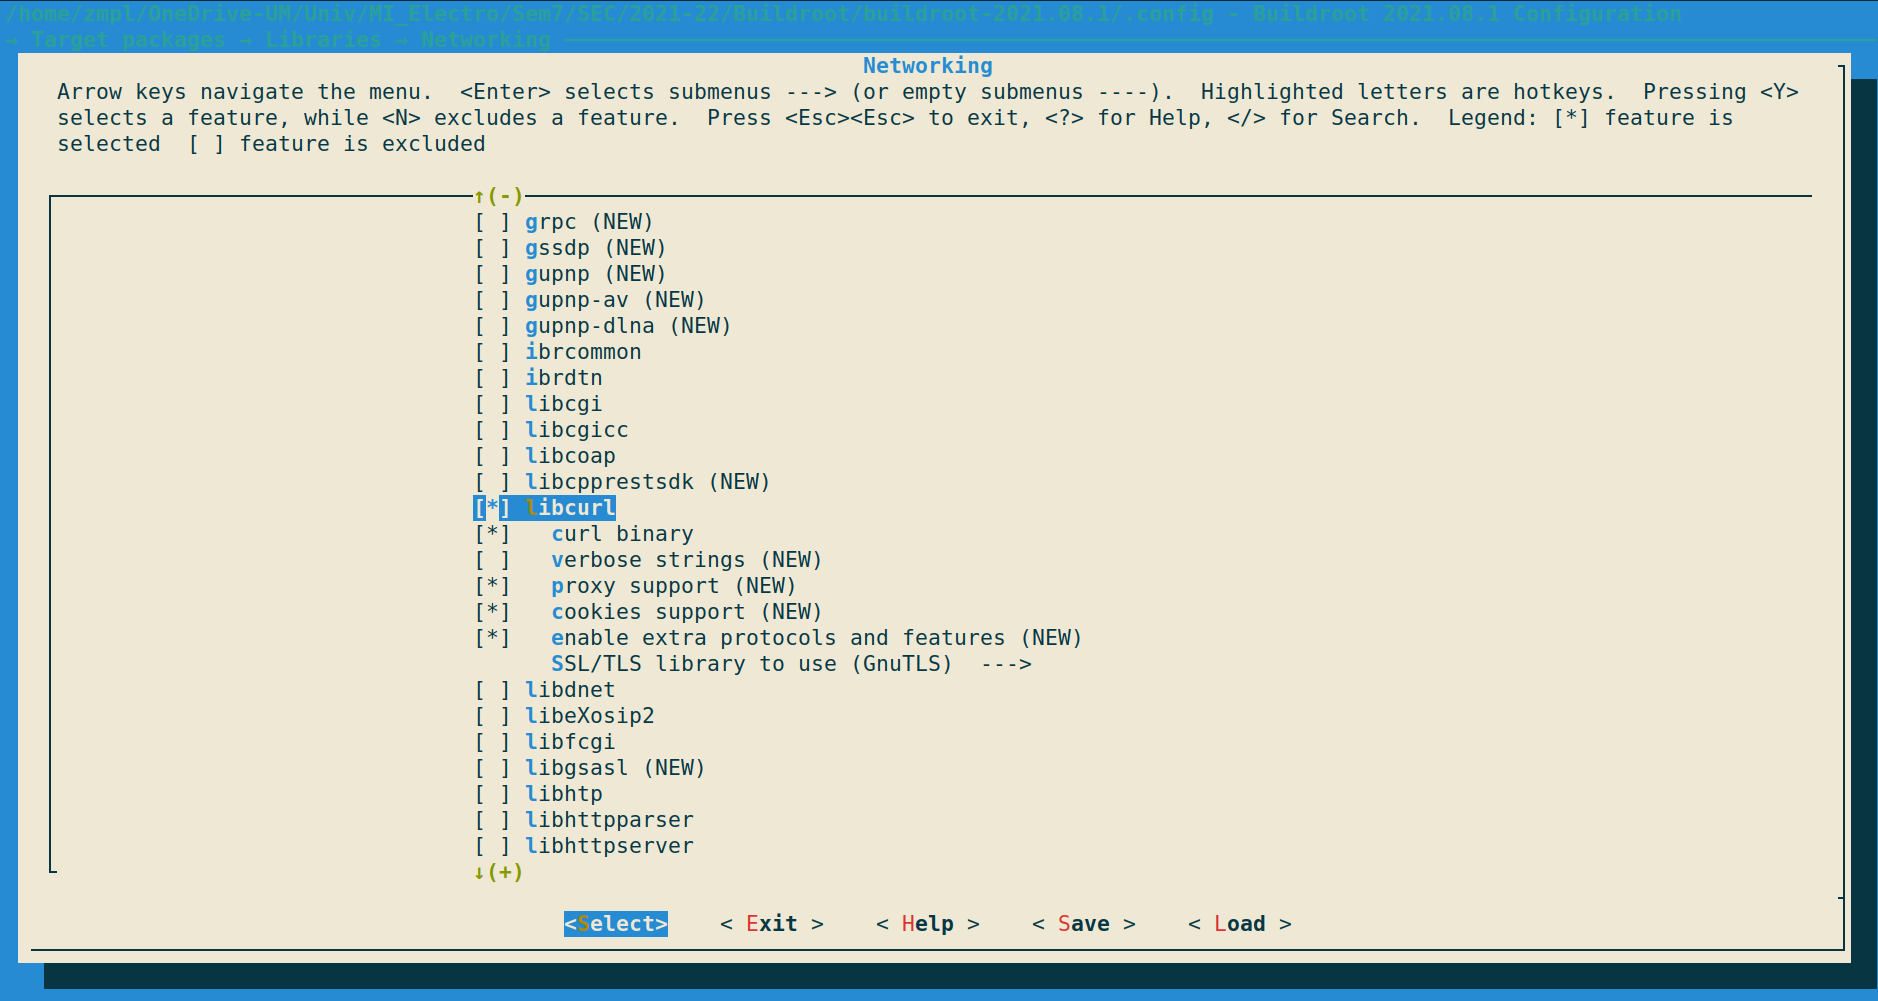
\includegraphics[width=0.8\columnwidth]{./img/buildroot-cfg-1.png}
  \caption{Buildroot setup: libcurl}%
\label{fig:buildroot-cfg-1}
\end{figure}
% 
\begin{figure}[htb!]
\centering
    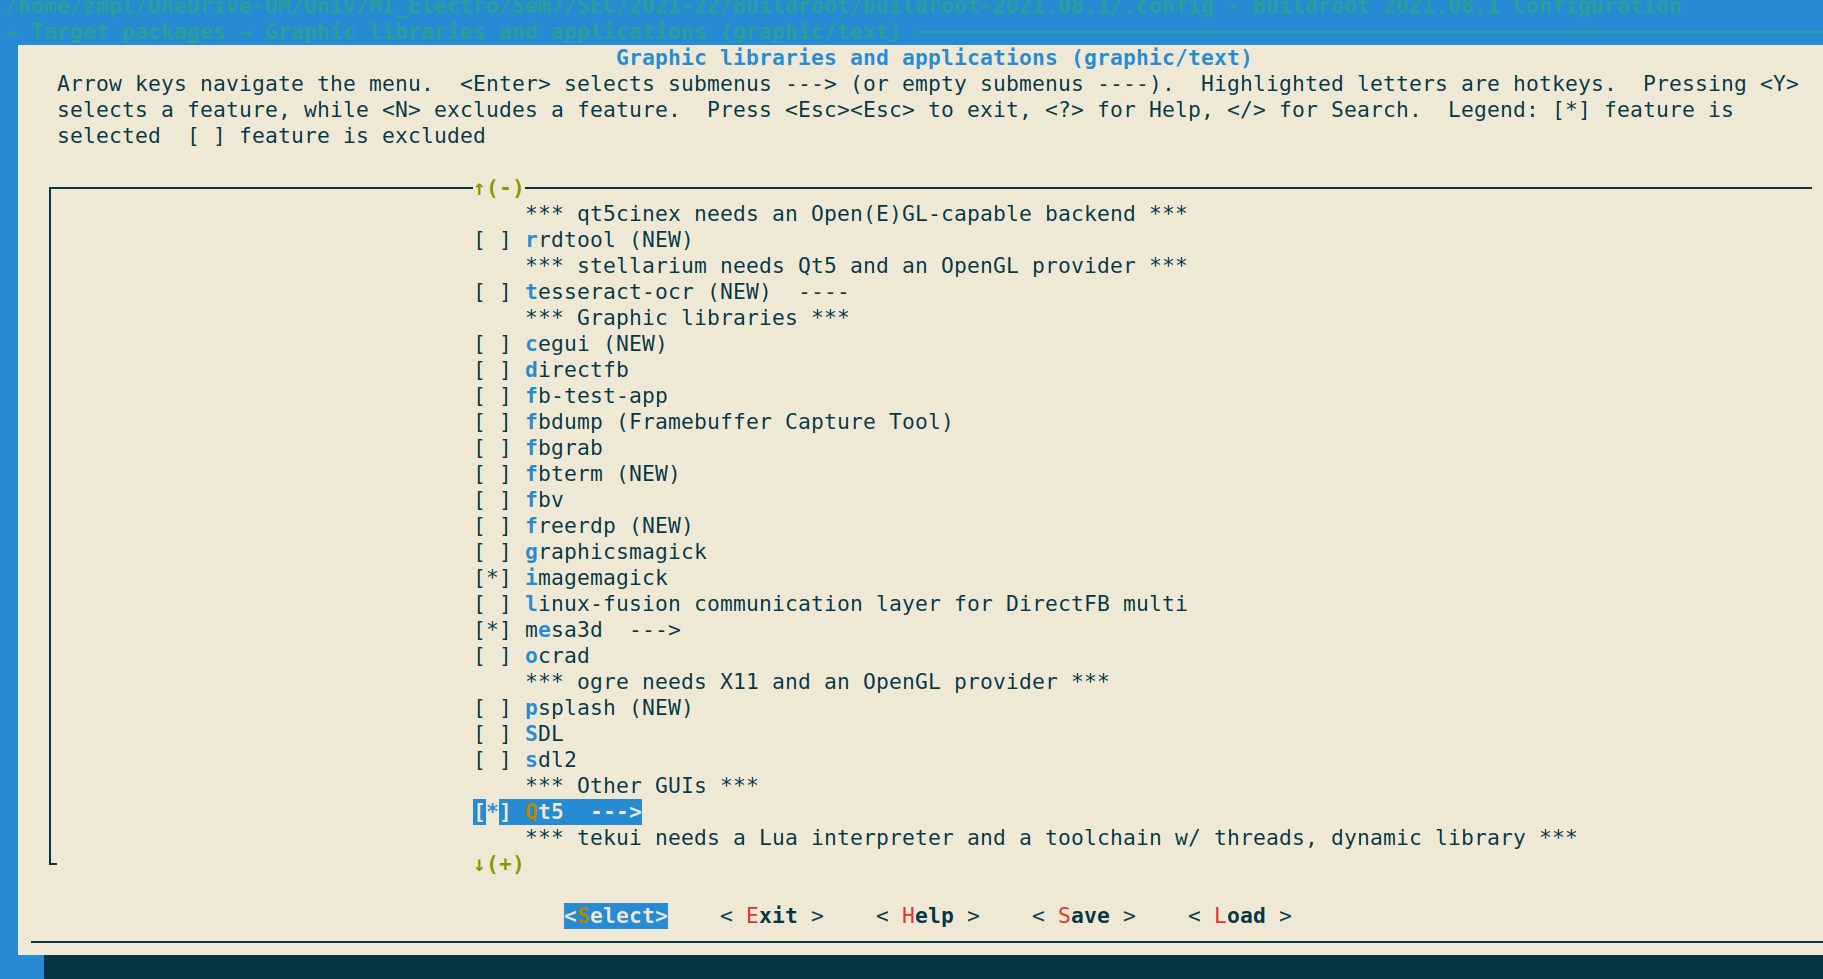
\includegraphics[width=0.8\columnwidth]{./img/buildroot-cfg-2.png}
  \caption{Buildroot setup: Qt5}%
\label{fig:buildroot-cfg-2}
\end{figure}
% 
\begin{figure}[htb!]
\centering
    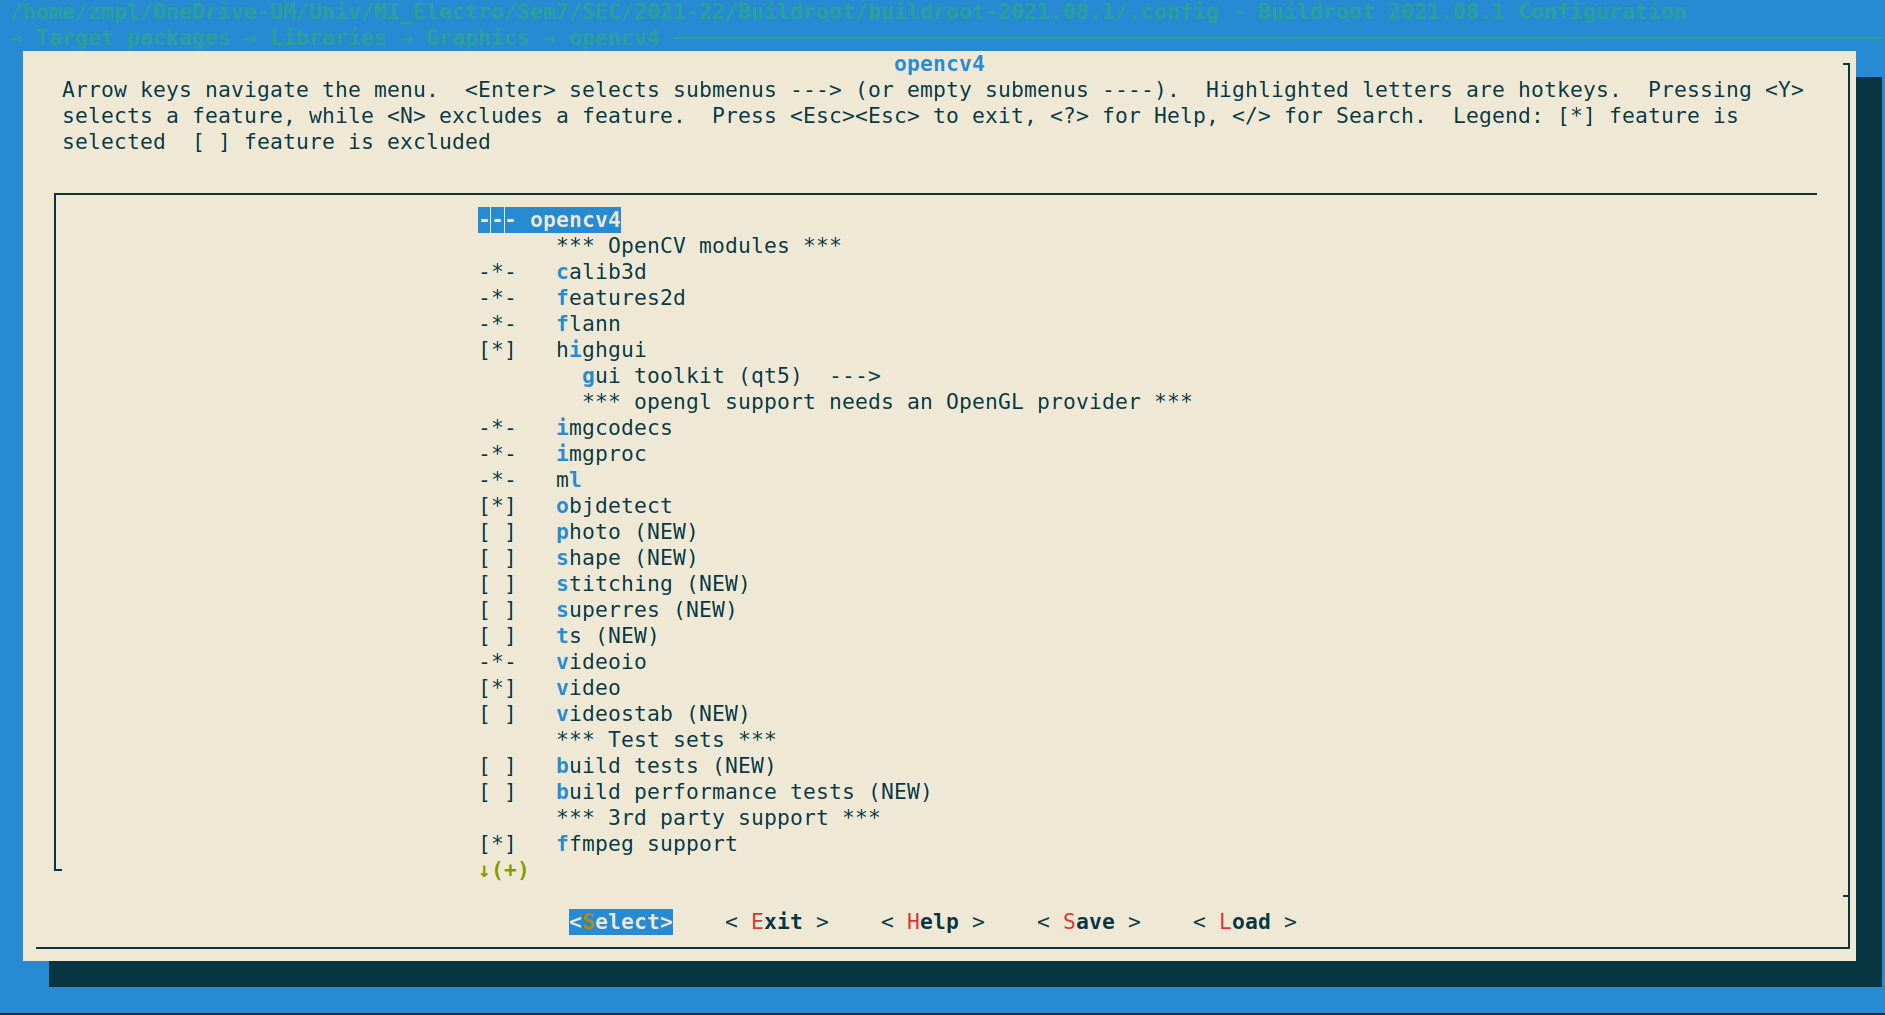
\includegraphics[width=0.8\columnwidth]{./img/buildroot-cfg-3.png}
  \caption{Buildroot setup: Opencv4}%
\label{fig:buildroot-cfg-3}
\end{figure}
% 
\begin{figure}[htb!]
\centering
    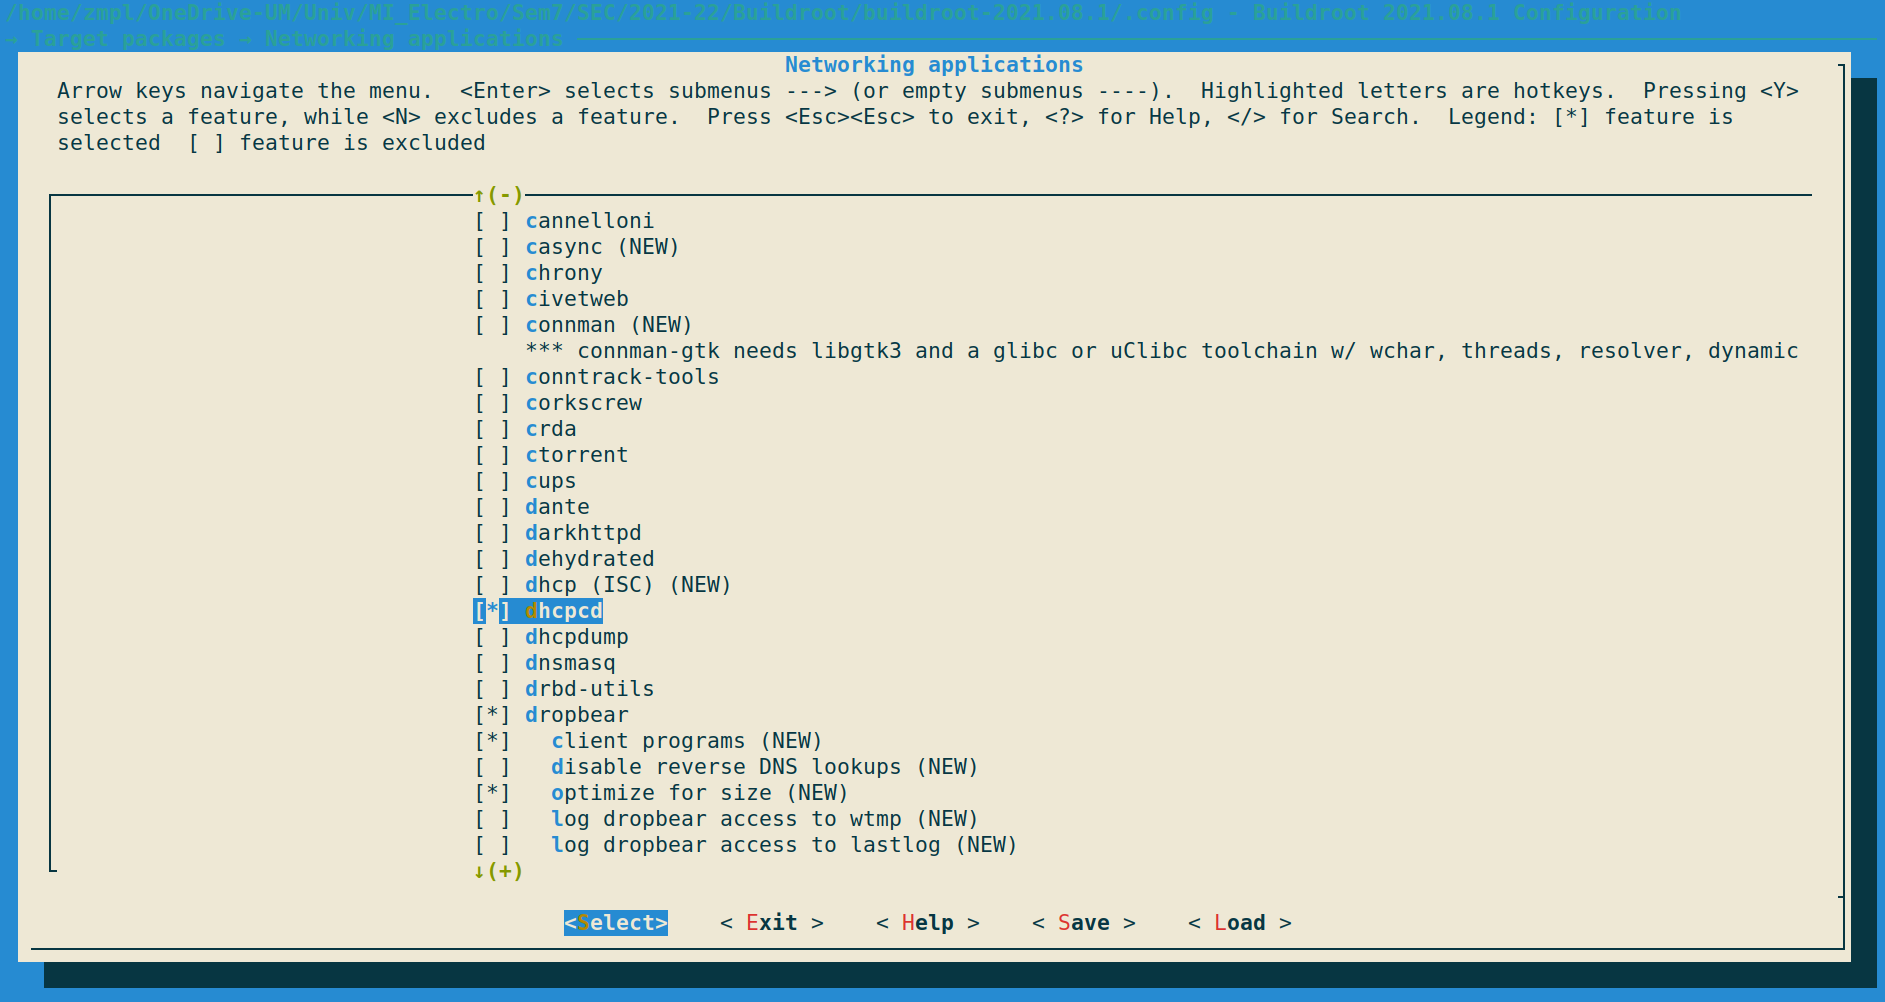
\includegraphics[width=0.8\columnwidth]{./img/buildroot-cfg-4.png}
  \caption{Buildroot setup: Networking}%
\label{fig:buildroot-cfg-4}
\end{figure}


\subsection{Automated build system for Local system software}
\label{sec:buildr-conf}
To build the \texttt{Local System} software an automated build tool was used,
namely \texttt{CMake}. \texttt{CMake} is a cross-platform tool to control the
software compilation process using platform and compiler independent
configuration files, and generating native \texttt{makefiles} to be executed,
building the required targets. For this purpose, a \texttt{CMakeLists.txt}
configuration file must be created in the software's path, as illutrated in Listing~\ref{lst:cmake-main}.

\lstinputlisting[language=c,
%firstline=1, lastline=3,
caption={\texttt{CMakeLists.txt} file: main build configuration file},
label=lst:cmake-main,
style=customc]{./listing/CMakeLists.txt}

Additionally, \texttt{CMake} provides better cross-compilation capabilities, by
enabling the programmer to specify the path to a toolchain configuration file,
keeping the original file general and delegating the specific compilation tools
for this file, as illustrated in Listing~\ref{lst:cmake-toolchain}.

\lstinputlisting[language=c,
%firstline=1, lastline=3,
caption={\texttt{raspToolchain.cmake} file: toolchain setup file},
label=lst:cmake-toolchain,
style=customc]{./listing/rasptoolchain.cmake}


%%% Local Variables:
%%% mode: latex
%%% TeX-master: "../../../dissertation"
%%% End:

\subsection{System initialization}
\label{sec:syst-init}
Embedded systems are typically self-contained and must be started without human
intervention, thus requiring an initialization scripted. The \texttt{inittab}
file contains the initialization scripts. In this file a line is added to
redirect to the initialization script of the \texttt{Local system}.
The process is relatively straightforward: adding modules to the \texttt{Linux}
kernel, setting up \gls{ipc} communication mechanisms like messages queues,
inserting the device driver modules into the \texttt{Linux} kernel, starting
daemons, running initialization commands (e.g., rotating the screen view), and
finally launching the main application.

\lstinputlisting[language=bash,
%firstline=1, lastline=3,
caption={Initialization script},
label=lst:init-sh,
style=make-pretty]{./listing/S_LS_Init.sh}

\subsection{Device drivers}
\label{sec:device-drivers-1}
Two device drivers were developed/adapted for fragrance diffusion and user
detection using two ultrasonic sensors. The device driver for user detection is
instantiated twice (in different \gls{hw} pins obviously), and then a daemon is
responsible to read periodically from these device drivers and assert if an user
was detected by counting these events in a sliding time window.

\subsubsection{Fragrance diffusion}
\label{sec:fragrance-diffusion}
The fragrance diffusion device driver must write to a specific pin to
enable/disable the device. The pin is statically defined in the module, thus
requiring recompilation for several diffuser actuators. In the future, this
should be changed to provide a more versatile interface. The module contains all
the typical functions associated with \texttt{static struct file\_operations},
namely \texttt{read}, \texttt{write}, \texttt{close} and \texttt{open}, although
the first is not required. The most important function is the \texttt{write}
one, which, upon writing to the associated file descriptor, sets the associated
pin state to \texttt{0} or \texttt{1}.
An excerpt of this device is illustrated
in Listing~\ref{lst:frag-module}.

\lstinputlisting[language=c,
%firstline=1, lastline=3,
caption={Fragrance diffuser kernel module (excerpt)},
label=lst:frag-module,
style=customc]{./listing/DDrivers/Frag/fragmodule.c}

\subsubsection{Ultrasonic sensor}
\label{sec:ultrasonic-sensor}
A device driver was implemented for the ultrasonic sensor, which can be
instantiated multiple times (in this case two), requiring the trigger and echo
pins, and the associated timeout. This device driver operates by emitting a
trigger signal and measuring the time between the trigger and echo signal to
determine the time of flight, and consequently the distance. Thus, this device
driver requires a specific signal timing as aforementioned in
Section~\ref{sec:motion-detection}..

The device driver implemented was adapted
from~\cite{hc-sro4-dd}, being ported to a more updated version, and abstracting
it. The most important functions are shown in
Listing~\ref{lst:uss-module}. Multiple device drivers can be instantiated or
removed in different hardware pins on demand, providing a more flexible
interface through the \texttt{sysfs\_configure\_store} function.
Then, on the background a periodic task performs the measurement ---
\texttt{do\_measurement} --- and when the echo is triggered a signal an
interruption is issued to handle this event, flushing the result to the
associated file descriptor.

It should be noted that for the present use case both triggers are shared,
as we expect to have `simultaneous' readings to work with.

\lstinputlisting[language=c,
%firstline=1, lastline=3,
caption={Ultrasonic sensor kernel module (excerpt) --- adapted from~\cite{hc-sro4-dd}},
label=lst:uss-module,
style=customc]{./listing/DDrivers/USS/hc-sro4.c}

\subsection{Daemons}
\label{sec:daemons-1}
As aforementioned, a daemon was created to periodically read the ultrasonic
sensors and count the detection events in a time sliding window, defining such
event as both sensors must be enabled. The daemon follows the required
initialization steps to detach itself from the outside world, as mentioned in
Section~\ref{sec:daemons}. Next, the message queue associated with the daemon is destroyed if present and
then (re)created.
Then, it should read the sensors periodically,
applying a sliding window and signaling the user detection event to a message
queue shared with the main application. The main application should periodically
consume this information to trigger the appropriate event handling. This daemon
is illustrated in Listing~\ref{lst:uss-daemon}.

\lstinputlisting[language=c,
%firstline=1, lastline=3,
caption={User detection daemon},
label=lst:uss-daemon,
style=customc]{./listing/Daemon/ussdaemon.cpp}

\subsection{Classes}
\label{sec:classes}
In these sections the main classes for the \texttt{Local System} are discussed.

\subsubsection{UI}
\label{sec:ui}
The \gls{ui} classes handle the interaction between the user and the application
and are defined according to the application mode, namely:
\begin{item-c}
\item \texttt{MainWindow}: main application's window. Manages all other windows
  (views), being the controller. The other views emit signals that are handled
  by these class to avoid circular dependencies and centralize the control.
\item \texttt{NormalWindow}: handles the Normal Window view application logic.
\item \texttt{InterWindow}: handles the Interaction Window view application logic.
\item \texttt{ImgFilterWindow}: handles the Image Filtering view application
  logic.
\item \texttt{SharWindow}: handles the Sharing view application logic.
\end{item-c}

In order to ease this model of control, the subordinate views are restricted to
a small subset of the application window, i.e., the only part that actually
requires replacing in each view. This means that the canvas to display the
images and the status bar is preserved throughout the application and solely
belongs to the \texttt{MainWindow}.

\paragraph{\textbf{NormalWindow}}
An example of a subordinate view is the \texttt{NormalWindow} which interface is
presented in Listing~\ref{lst:norm-wind}. It can be seen that it contains
a \texttt{Qt signal} to indicate when \texttt{Normal view} must be exited, and
it was used to test the application logic. This \texttt{Qt signal} is then
connected to the callback of a recipient object (a \texttt{slot}) to perform
some action.

\lstinputlisting[language=c,
%firstline=1, lastline=3,
caption={\texttt{NormalWindow} --- an example of a subordinate view},
label=lst:norm-wind,
style=customc]{./listing/LSApp/normalwindow.h}

\paragraph{\textbf{MainWindow}}
It is the view controller and the application logic manager, holding the
definition for each of the modes.
Listing~\ref{lst:main-wind} presents the interface for this class.

\lstinputlisting[language=c,
%firstline=1, lastline=3,
caption={\texttt{MainWindow} --- interface},
label=lst:main-wind,
style=customc]{./listing/LSApp/mainwindow.h}

It is
composed of several objects, namely:
\begin{item-c}
\item subordinate views (windows);
\item video capture
\item threads
\item mutexes: for synchronization
\item pEvents: wrapper around condition variables; for synchronization
\item image filters
\item scenes: welcome, video, and interaction
\item GIF
\item Twitter
\item Post: Twitter post
\item Video Player
\item Ad: current ad
\item Fragrance: current fragrance, fragrance manager to determine fragrance
  settings from the database, a diffuser and the associated timer for actuation
\item Timer: for periodic tasks
\item Socket: to connect to remote system
\item Message queue to interface the user detection sensors via daemon
\end{item-c}

It provides functions to:
\begin{itemize}
\item handle subordinate views signals and other relevant events like taking a
  picture, sharing a post, connection to the remote, receiving data from remote
  system, etc.
\item Handle computer vision tasks: grab frames, display images, detect faces,
  recognize gestures to navigate the interface and apply filters.
\item Thread workers: functions associated to each thread.
\item Twitter authentication
\item GIF creation
\item Handling communication
\item and several helpers
\end{itemize}

The threads and the associated workers will be detailed later.

\subsubsection{Ad}
\label{sec:ad}
This class handles ad logic, namely (see Listing~\ref{lst:ad}):
\begin{item-c}
\item storing relevant data
\item saving to and restoring data from the database
\item Retrieving important data like the filterID, the fragID, the timeslot, or
  the enabled state.
\item Enabling the Ad, dispatching it for execution in the normal mode,
  obviously if there is no user interaction.
\end{item-c}
It is important to note that this class is thread safe as it includes a
synchronization mechanism --- a mutex --- to prevent unattended access.

\lstinputlisting[language=c,
%firstline=1, lastline=3,
caption={\texttt{Ad} --- interface},
label=lst:ad,
style=customc]{./listing/LSApp/ad.h}

\subsubsection{DigitalOutput}
\label{sec:digitaloutput}
This class, enclosed in the \texttt{Device::Driver} namespace, models a digital
output device driver, as the fragrance diffuser. It provides methods to open,
write and close the device driver, as illustrated in Listing~\ref{lst:ddDigitalOut}.

\lstinputlisting[language=c,
%firstline=1, lastline=3,
caption={\texttt{DigitalOut} --- interface},
label=lst:ddDigitalOut,
style=customc]{./listing/LSApp/ddDigitalOut.h}

\subsubsection{Fragrance classes}
\label{sec:fragrance-classes}
The fragrance classes, enclosed in the \texttt{Fragrance} namespace, handle the
fragrance logic, namely, creating, diffusing and managing it.

\paragraph{\textbf{Frag}}
The \texttt{Frag} class defines a Fragrance as illustrated in
Listing~\ref{lst:frag}. It allows to calculate the durations of the enabled and
disabled state of the fragrance diffuser associated with it, and besides the
normal getters and setters, it provides methods to serialize and deserialize
this object, enabling it to be saved and loaded from the database.

\lstinputlisting[language=c,
%firstline=1, lastline=3,
caption={\texttt{Frag} --- interface},
label=lst:frag,
style=customc]{./listing/LSApp/frag.h}

\paragraph{\textbf{fragDiffuser}}
The fragrance diffuser class associates a fragrance with the respective device
driver, enabling it to appropriately handle the requirements of each
fragrance (see Listing~\ref{lst:fragDiffuser}).
It is important to note that this class is thread safe as it includes a
synchronization mechanism --- a mutex --- to prevent unattended access.

\lstinputlisting[language=c,
%firstline=1, lastline=3,
caption={\texttt{fragDiffuser} --- interface},
label=lst:fragDiffuser,
style=customc]{./listing/LSApp/fragDiffuser.h}

\paragraph{\textbf{fragManager}}
The \texttt{FragManager} classes manages the fragrance database containing its
settings (see Listing~\ref{lst:fragManager}).
It is important to note that this class is thread safe as it includes a
synchronization mechanism --- a mutex --- to prevent unattended access.

\lstinputlisting[language=c,
%firstline=1, lastline=3,
caption={\texttt{fragManager} --- interface},
label=lst:fragManager,
style=customc]{./listing/LSApp/fragManager.h}

\subsubsection{ImgFilter}
\label{sec:imgfilter}
The \texttt{ImgFilter} class wraps the image filter functionality, mainly as a
container
(see Listing~\ref{lst:imgFilter}).

\lstinputlisting[language=c,
%firstline=1, lastline=3,
caption={\texttt{imgFilter} --- interface},
label=lst:imgFilter,
style=customc]{./listing/LSApp/imgfilter.h}

\subsubsection{msgQueue}
\label{sec:msgqueue}
The \texttt{msgQueue} class provides an abstraction over the Linux system calls
to ease the usage of this \gls{ipc} mechanism
(see Listing~\ref{lst:mqueue}).

\lstinputlisting[language=c,
%firstline=1, lastline=3,
caption={\texttt{msgQueue} --- interface},
label=lst:mqueue,
style=customc]{./listing/LSApp/msgqueue.h}

\subsubsection{pEvent}
\label{sec:msgqueue}
The \texttt{pEvent} class provides an abstraction over the pthread condition
variables, comprising the loosely named POSIX Event. This class enables to emit
and receive signals in a much more straightforward way, but always ensuring its
integrity, as it is protected by a mutex
(see Listing~\ref{lst:pEvent}).

\lstinputlisting[language=c,
%firstline=1, lastline=3,
caption={\texttt{pEvent} --- interface},
label=lst:pEvent,
style=customc]{./listing/LSApp/pEvent.h}

\subsubsection{Post}
\label{sec:post}
The \texttt{Post} class handles the Twitter posts, containing the message and
the associated media type
(see Listing~\ref{lst:post}).

\lstinputlisting[language=c,
%firstline=1, lastline=3,
caption={\texttt{Post} --- interface},
label=lst:post,
style=customc]{./listing/LSApp/post.h}

\subsection{Threads}
\label{sec:threads}
This section addresses the Local System threads, illustrated in Listing~\ref{lst:threads}.

\lstinputlisting[language=c,
%firstline=1, lastline=3,
caption={Local system threads},
label=lst:threads,
style=customc]{./listing/LSApp/threads.cpp}

\subsubsection{frameGrab}
\label{sec:framegrab}
The \texttt{frameGrab} thread is responsible for acquiring a camera frame and
feeding the computer vision engine to detect faces, recognize gestures, or apply
image filters. It checks the mode and if adequate the frame is captured and
dispatched for further processing.

\subsubsection{Rx and ProcessRx}
\label{sec:rx}
The \texttt{Rx} and \texttt{ProcessRx} threads work together following the
producer--consumer model: the first receives data frames from the Remote System
and pushes it to a shared buffer, signaling this event to the \texttt{ProcessRx}
thread;
the second consumes these data frames, parsing them, and signaling the relevant
events, like downloading an Ad.

\subsubsection{gifSave}
\label{sec:gifsave}
The \texttt{gifSave} thread takes care of saving a GIF into disk. A thread is
required because this I/O operation can take a significant amount of time.

\subsubsection{DownloadAd}
\label{sec:downloadad}
The \texttt{downloadAd} thread takes care of downloading an ad and the
associated media through the proxy server \texttt{transfer.sh}. When the event
\texttt{ev\_download} is signaled, the current ad is retrieved and the ad is downloaded.

\subsubsection{Main thread}
\label{sec:main-thread}
The main thread belongs to the \texttt{UI}, and it responsible for processing
its events. Associated with this thread, a periodic task is executed to verify
the application mode and stimulate the application (see
Listing~\ref{lst:periodicTask}), namely: checking normal mode, checking if a
user was detected, or if a remote connection was lost.

\lstinputlisting[language=c,
%firstline=1, lastline=3,
caption={Main thread periodic task: checkMode},
label=lst:periodicTask,
style=customc]{./listing/LSApp/periodicTask.cpp}


\section{Deployment}
\label{sec:deployment}
As aforementioned the implementation of the Local System was performed and
tested on the host before cross-compiling and deploying to the target embedded
system.

However, and even though a successful target system image was obtained, the deployment was not possible as the cross-compiling revealed itself
more complicated due to the dependency on external libraries.

Nonetheless, as the application logic was successfully validated, the deployment
task resides only on the successful cross-compiling which could not be attended
due to time restrictions.
%%% Local Variables:
%%% mode: latex
%%% TeX-master: "../../../dissertation"
%%% End:
